%! TeX program = lualatex
\documentclass[12pt,t]{beamer}
\usepackage{graphicx}

% % get rid of junk
% \usetheme{default}
% \beamertemplatenavigationsymbolsempty
% \hypersetup{pdfpagemode=UseNone} % don't show bookmarks on initial view

% Strikethrough 
\usepackage[normalem]{ulem}


% UK dates
\usepackage[UKenglish]{babel}% http://ctan.org/pkg/babel
\usepackage[UKenglish]{isodate}% http://ctan.org/pkg/isodate
\cleanlookdateon % Remove ordinal day reference

% font
\usepackage{fontspec}
\setsansfont{TeX Gyre Heros}
\setbeamerfont{note page}{family*=pplx,size=\footnotesize} % Palatino for notes

% named colors
\definecolor{offwhite}{RGB}{24,24,24 }
\definecolor{background}{RGB}{226, 218, 218}

\definecolor{title}{RGB}{104, 36, 109}
% \definecolor{title}{RGB}{55, 0, 117}
\definecolor{subtitle}{RGB}{98, 0, 151}

\definecolor{foreground}{RGB}{0, 0, 0}
\definecolor{hilight}{RGB}{104, 36, 109}

\definecolor{gray}{RGB}{104, 36, 109}
\definecolor{vhilight}{RGB}{120, 0, 0}
\definecolor{lolight}{RGB}{155,155,155}

% use those colors
\setbeamercolor{titlelike}{fg=title}
\setbeamercolor{subtitle}{fg=subtitle}
\setbeamercolor{institute}{fg=hilight}
\setbeamercolor{normal text}{fg=foreground,bg=background}
\setbeamercolor{item}{fg=foreground} % color of bullets
\setbeamercolor{subitem}{fg=gray}
\setbeamercolor{itemize/enumerate subbody}{fg=gray}
\setbeamertemplate{itemize subitem}{{\textendash}}
\setbeamerfont{itemize/enumerate subbody}{size=\footnotesize}
\setbeamerfont{itemize/enumerate subitem}{size=\footnotesize}

% % page number
% \setbeamertemplate{footline}{%
%     \raisebox{5pt}{\makebox[\paperwidth]{\hfill\makebox[20pt]{\color{hilight}
%           \scriptsize\insertframenumber}}}\hspace*{5pt}}

% add a bit of space at the top of the notes page
\addtobeamertemplate{note page}{\setlength{\parskip}{12pt}}

% a few macros
\newcommand{\bi}{\begin{itemize}}
\newcommand{\ei}{\end{itemize}}
\newcommand{\ig}{\includegraphics}
\newcommand{\subt}[1]{{\footnotesize \color{subtitle} {#1}}}

% \usepackage{color}
\definecolor{Red}{cmyk}{0,1,1,0}
\def\red{\color{Red}}

% title info
\title{{\Huge Git your sheet together} \\ Git for mathematical writing}
\author{\href{http://lchiarini.com}{Leandro Chiarini}}
\institute{Durham University}
\date{\today \\
	\vspace{2em}
}

\begin{document}

% title slide
{
\setbeamertemplate{footline}{} % no page number here
\frame{ \titlepage
   } }


\begin{frame}{Why Version Control?}
\begin{itemize}
		\pause
		\vspace{1em}
    \item Track changes 
		\pause
		\vspace{1em}
    \item Collaborate effectively 
		\pause
		\vspace{1em}
    \item Revert to previous versions/and explore new ideas
		\pause
\end{itemize}

\end{frame}

\begin{frame}{Example with pictures}
	{\red todo}
	% %
	% \begin{figure}[ht]
	%     \centering
	% 		\only<1>{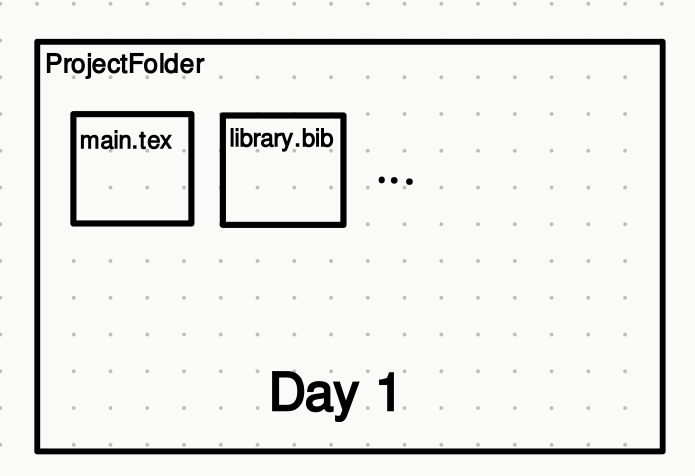
\includegraphics[width=0.6\textwidth]{figs/Day1.png}}
	% 		\only<2>{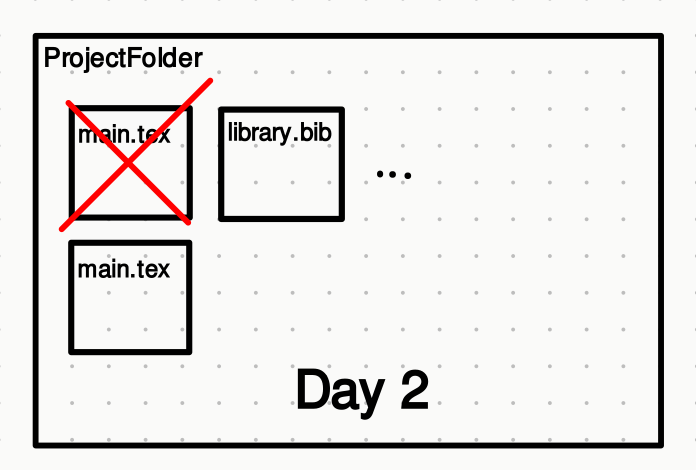
\includegraphics[width=0.6\textwidth]{figs/Day2.png}}
	% 		\only<3>{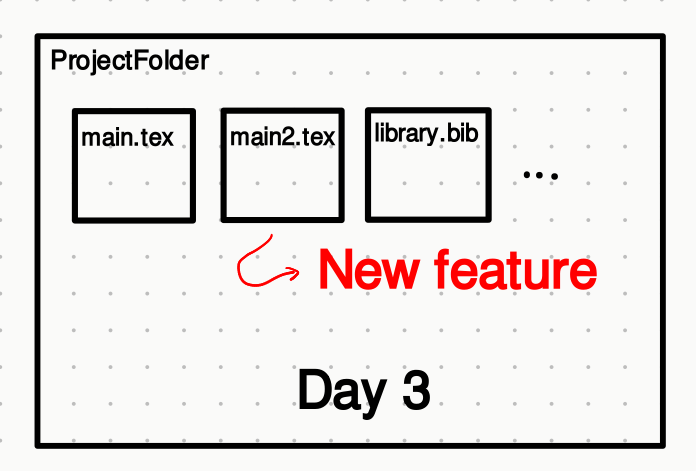
\includegraphics[width=0.6\textwidth]{figs/Day3.png}}
	% 		\only<4>{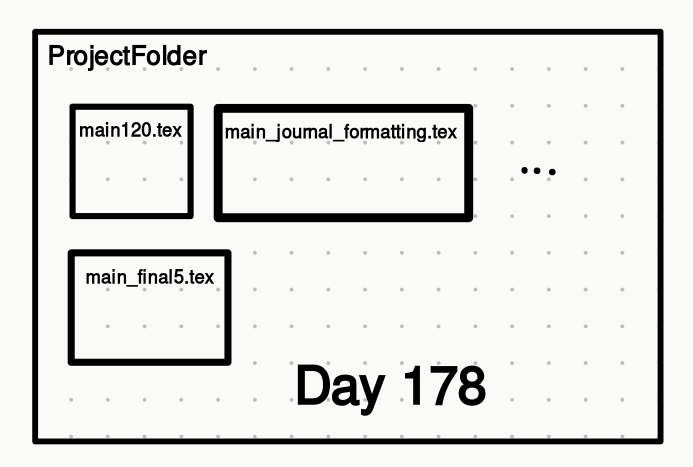
\includegraphics[width=0.6\textwidth]{figs/Day178.png}}
	% \end{figure}
	% %
\end{frame} 

\begin{frame}\frametitle{Git}
%
\pause
\begin{figure}[ht]
    \centering
    
\includegraphics[width=0.4\textwidth]{figs/git-xkcd-comic.png}
	\caption{xkcd Comic about Git}
\end{figure}
%
\end{frame}

% \begin{frame}{What is different about Git?}
% 	\vspace{1em}
% 	Example:
% 	\begin{figure}[ht]
% 		\centering
% 		\includegraphics[width=0.6\textwidth]{figs/git-graph-example.png}
% 		\caption{Git acyclic directed graph structure
% 		\\ image by https://salferrarello.com/}
% 	\end{figure}
% \end{frame}

\begin{frame}{What is different about Git?}
	\vspace{1em}
	Example:
	\pause
	{\red to do}
	\pause
\begin{itemize}
	\vspace{1em}
    \item Control what/when changes to be tracked
		\vspace{1em}
		\pause
	\item Records snapshots of your project as a \only<4>{``tree''} \pause \only<5->{\textit{acyclic directed graph}}
		\vspace{1em}
		\pause
	\item Works especially well with plain text files \pause (\LaTeX)
		\pause 
		\vspace{1em}
		\begin{itemize}
			\item To save all your photos, better use something else.
		\end{itemize}
\end{itemize}
\end{frame}

\begin{frame}{Basic Workflow}
\begin{itemize}
	\item 
	\only<-2>{\texttt{git init}:}\pause \only<-2>{ start a new repository}
		\only<3->{\sout{\texttt{git init}: start a new repository}}
		\pause
		\vspace{1em}
    \item \texttt{git clone <url>}:  copy a git repository
		\pause
		\vspace{1em}
    \item \texttt{git add <files>}:  stage changes
		\pause
		\vspace{1em}
    \item \texttt{git commit -m "<message>"}: save changes as ``snapshot'' 
		\pause
		\vspace{1em}
    \item \texttt{git status}, \texttt{git log}, \texttt{git diff}
\end{itemize}
\end{frame}



\begin{frame}{Branches and merging}
\begin{itemize}
		\vspace{1em}
    \item \texttt{git checkout} 
		\pause
		\vspace{1em}
	\item \texttt{git branch}
		\pause
		\begin{itemize}
			\item Experiment without fear
				\pause
			\item Git via overleaf only allows for a single branch
				\pause 
		\end{itemize}
		\vspace{1em}
	\item \texttt{git merge}
		\pause
		\vspace{1em}
	\item \texttt{git stash}
		\pause
		\vspace{1em}
\end{itemize}
\end{frame}

\begin{frame}{Key Concepts}
\begin{itemize}
    \item Repository (repo)
		\pause
		\vspace{1em}
    \item \texttt{.git} folder
		\pause
		\begin{itemize}
			\item Do not put git inside of dropbox
		\end{itemize}
		\pause
		\vspace{1em}
    \item Commit and staging area
		\pause
		\vspace{1em}
	\item Remote vs local
		\pause
		\vspace{1em}
    \item Branches and merging
\end{itemize}
\end{frame}

% \begin{frame}{Undo Without Fear}
% \begin{itemize}
%     \item Revert to any point in history
% 		\pause
% 		\vspace{1em}
%     \item Branch to test new proof strategies
% 		\pause
% 		\vspace{1em}
%     \item Use \texttt{stash} to temporarily save changes
% 		\pause
% 		\vspace{1em}
%     \item Git makes experimenting safe!
% 		\pause
% 		\vspace{1em}
% \end{itemize}
% \end{frame}

% \begin{frame}{Branches for Experiments}
% \begin{itemize}
%     \item Try out changes on separate branches
% 		\pause
% 		\vspace{1em}
%     \item Merge back once satisfied
% 		\pause
% 		\vspace{1em}
%     \item Keep main branch stable
% 		\pause
% 		\vspace{1em}
%     \item Resolve merge conflicts with care
% \end{itemize}
% \end{frame}

\begin{frame}{Best Practices for git with \LaTeX}
\begin{itemize}
    \item Use one sentence per line
		\pause
		\vspace{1em}
    \item Ignore build files with \texttt{.gitignore}
		\pause
		\vspace{1em}
    \item Commit logically grouped changes
		\pause
		\vspace{1em}
    \item Write meaningful commit messages
\end{itemize}
\end{frame}

\begin{frame}{Collaborating with Git}
\begin{itemize}
    \item Pull requests (PRs) for review
		\vspace{1em}
		\pause
    \item Review diffs of mathematical arguments
		\vspace{1em}
		\pause
    \item Assign co-author responsibilities
		\vspace{1em}
		\pause
    \item Write good commit messages
\end{itemize}
\end{frame}

\begin{frame}{Tooling and Interfaces}
\begin{itemize}
    \item GitHub Desktop, GitKraken, SourceTree
		\vspace{1em}
		\pause
    \item Overleaf Git integration
		\vspace{1em}
		\pause
    \item Diff tools: \texttt{latexdiff}, \texttt{diffpdf}
\end{itemize}
\end{frame}

\begin{frame}{Practical Exercise}
\begin{itemize}
    \item Initialise a repo for a paper
		\vspace{1em}
		\pause
    \item Make edits and commit
		\vspace{1em}
		\pause
    \item Create and merge a branch
		\vspace{1em}
		\pause
    \item View commit history
\end{itemize}
\end{frame}

\begin{frame}[allowframebreaks]\frametitle{Some references}
\nocite{*}
\bibliographystyle{abbrv}
\bibliography{library}
\end{frame}

		
\end{document}
